\documentclass[
]{jss}

\usepackage[utf8]{inputenc}

\providecommand{\tightlist}{%
  \setlength{\itemsep}{0pt}\setlength{\parskip}{0pt}}

\author{
H. Sherry Zhang\\Monash University \And Dianne Cook\\Monash University
\AND Ursula Laa\\University of Natural Resources and Life Sciences
\AND Nicolas Langrené\\CSIRO Data61 \AND Patricia
Menéndez\\Monash University \AND
}
\title{\pkg{cubble}: An R Package for Structuring Spatio-temporal Data}

\Plainauthor{H. Sherry Zhang, Dianne Cook, Ursula Laa, Nicolas
Langrené, Patricia Menéndez}
\Plaintitle{cubble: An R Package for Structuring Spatio-temporal Data}

\Abstract{
The abstract of the article.
}

\Keywords{spatio-temporal data, \proglang{R}}
\Plainkeywords{spatio-temporal data, R}

%% publication information
%% \Volume{50}
%% \Issue{9}
%% \Month{June}
%% \Year{2012}
%% \Submitdate{}
%% \Acceptdate{2012-06-04}

\Address{
          }

% Pandoc citation processing

% Pandoc header

\usepackage{amsmath} \usepackage{array}

\begin{document}

\newpage

\hypertarget{introduction}{%
\section{Introduction}\label{introduction}}

\textbf{Motivation}

Many data structures have been proposed for spatial (\texttt{sf} by
\citet{sf}) and temporal (\texttt{tsibble} by \citet{tsibble}) data in
the R community, while less has been done for spatio-temporal data. The
lack of such tools could potentially because analysts usually treat the
spatial and temporal dimension pf the data separately, without realising
the need to create a new data structure. While this approach follows the
third tidy data principal \citep{tidydata} (\emph{Each type of
observational unit forms a table}), analysts always need to manually
join results from different observational units or combining multiple
tables into one for downstream analysis. This additional step doesn't
add new operations into the data but can be error prone. \newline

\textbf{Existing packages}

Currently, available spatio-temporal data structure in R includes:
\texttt{spacetime}\citep{spacetime}, which proposes four space-time
layouts: Full grid (STF), sparse grid(STS), irregular (STI), and
trajectory (STT). The data structure it uses is based on \texttt{sp}
\citep{sp} and \texttt{xts}\citep{xts}, both of which has been replaced
by more recent implementations. \texttt{spatstat} \citep{spatstat}
implements a \texttt{ppp} class for point pattern data; and more recent,
\texttt{stars} \citep{stars} implements a spatio-temporal array with the
dplyr's data cube structure \texttt{cubelyr} \citep{cubelyr} as its
backend. While these implementations either store spatial and temporal
variables all in a single table, hence duplicate the spatial variables
for each temporal unit; or split them into two separate tables that has
the problem of manually joining, mentioned in the previously. None of
these packages enjoy both the benefits of being able to separate
manipulation in the two dimensions while also keep the data object as a
whole. This create a gap in the software development. The requirement
for such a tool is important given the ubiquity of spatio-temporal
vector data in the wild: the Ireland wind data from \texttt{gstat} is an
classic example data that splits variables into spatial
(\texttt{wind.loc}) and temporal (\texttt{wind}) dimension; Bureau of
Meteorology (BoM) provides climate observations that are widely applied
in agriculture and ecology study; air pollution data. \newline

\textbf{Our new data structure for spatio-temporal data}\\
This paper describes the implementation of a new spatio-temporal data
structure: \texttt{cubble}. \texttt{cubble} implements a relational data
structure that uses two forms to manage the switch between spatial and
temporal dimension. With this structure, users can manipulate the
spatial or temporal dimension separately, while leaves the linking of
two dimensions to \texttt{cubble}. The software is available from the
Comprehensive R Archive Network (CRAN) at {[}CRAN link{]}. \newline

\textbf{Section division}

The rest of the paper will be divided as follows: {[}complete when the
paper structure is more solid{]}

\newpage

\hypertarget{the-cubble-package}{%
\section{The cubble package}\label{the-cubble-package}}

Spatio-temporal data usually come in various forms and Figure
\ref{fig:cubble-diagram} shows four examples of this. No matter
whichever form the data is in, there are always some common components
shared by these data. A spatial identifier (\texttt{id} in the diagram)
identifies each site. The temporal identifier (\texttt{t} in the
diagram) {[}\ldots{]}. Coordinates, comprising of latitude and
longitude, are commonly used variables for point pattern data.These
identifiers will be the building blocks for the data structure
introduced below. For other variables, those invariant at each time
stamp are spatial variables and those differ are temporal variables.

\begin{CodeChunk}
\begin{figure}

{\centering 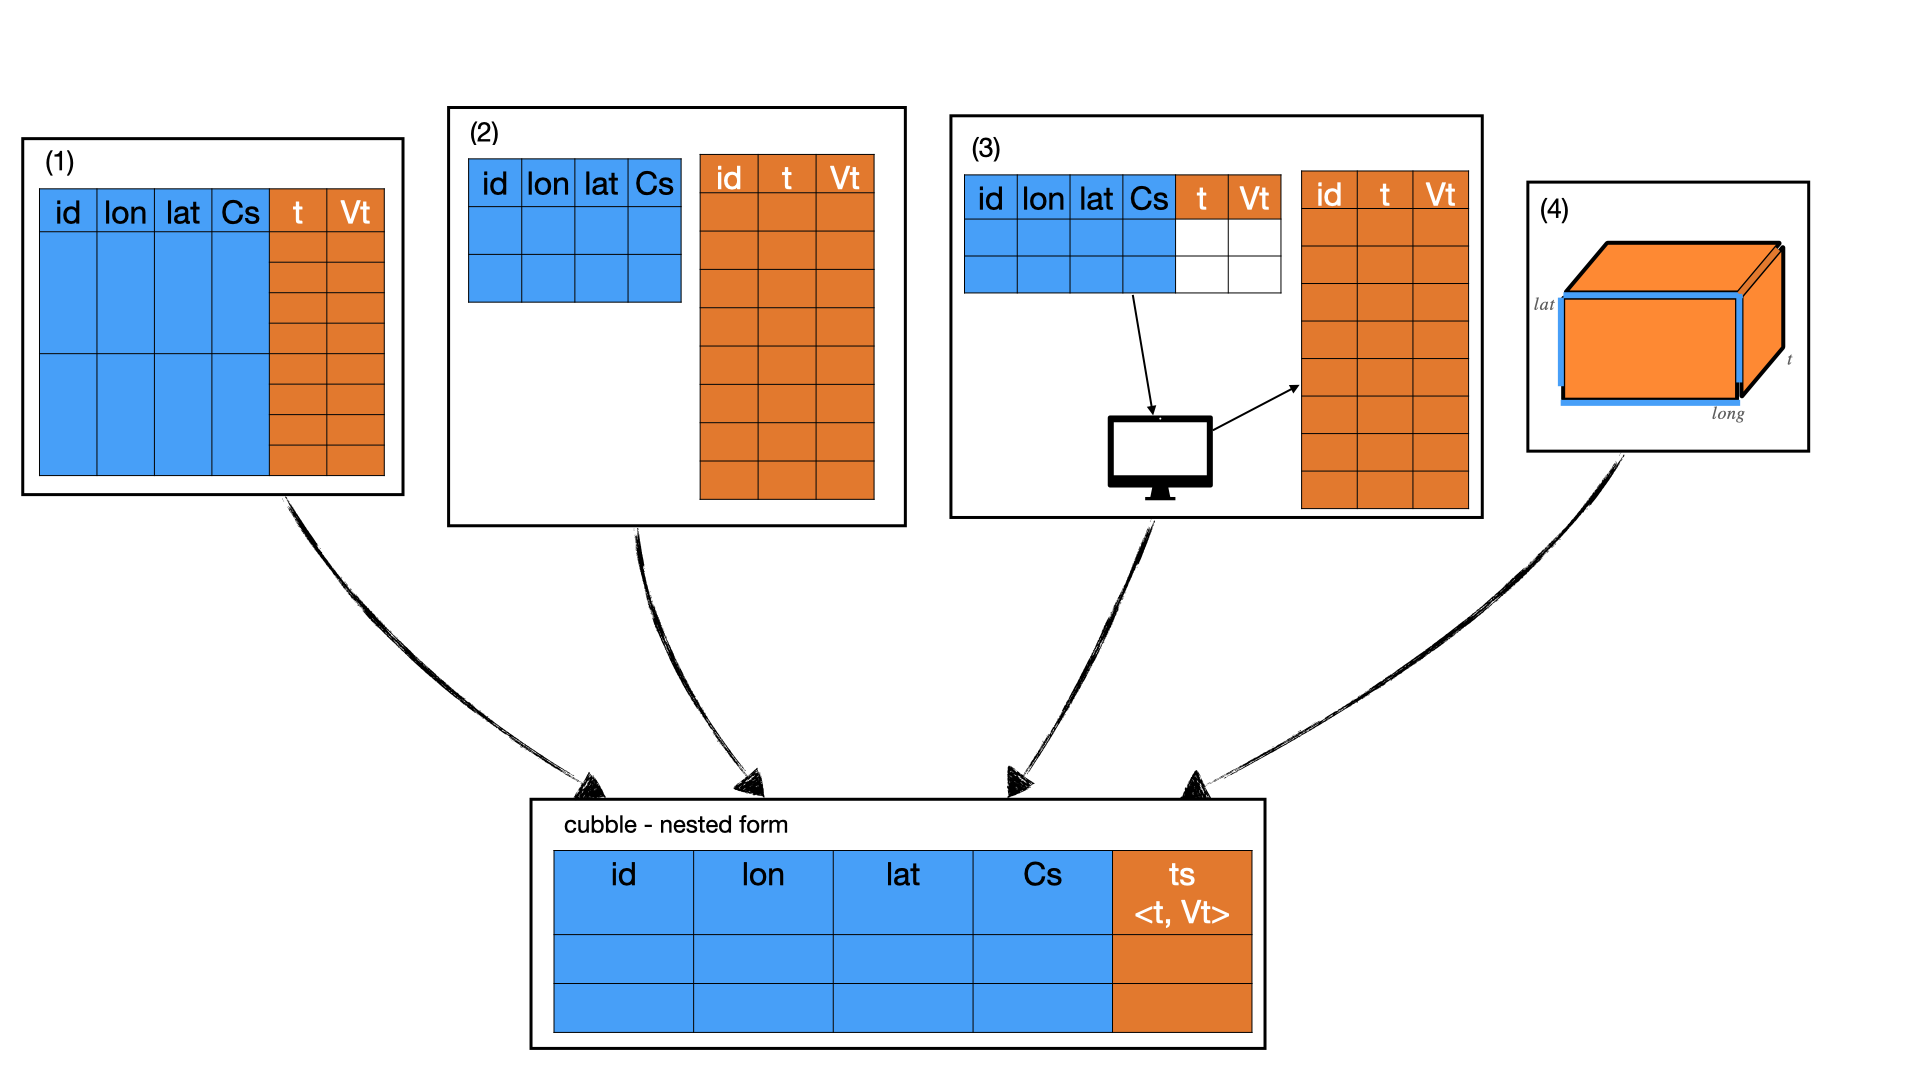
\includegraphics[width=1\linewidth,height=0.15\textheight]{/Users/sherryzhang/Documents/research/paper-cubble/figures/input-formats/input-formats.001} 

}

\caption[Illustration of incoming data formats for spatio-temporal data]{Illustration of incoming data formats for spatio-temporal data. (1) Data comes in as a single table; (2) Separate tables for spatial and temporal variables; (3) A single table with all the parameters used to query the database and a separate table for queried data; and (4) Cubical data in array or NetCDF format.}\label{fig:cubble-diagram}
\end{figure}
\end{CodeChunk}

In a cubble, there are two forms: 1) nested form, for manipulating the
spatial dimension, and 2) long form, for manipulating the temporal
dimension. Figure \ref{fig:def-cubble} sketches the two forms along with
the associated attributes. A variable identifies by the spatial
identifies can come from manipulating spatial variables itself, or
summary of temporal variables. The nested cubble is best suited to work
with this type of operation, since it defines each spatial unit as a
row. The spatial variables are directly displayed in columns. Temporal
variables are nested in a column called \texttt{ts} and the underlying
rowwise dataframe uses a \texttt{group} attributes to ensure each row is
in its own group.

Temporal operations are suited to be performed in the long cubble as
each row is defines as the combination of spatial and temporal
identifier. This is also the structure that \texttt{tsibble} adopts.
Temporal variables are directly displayed. To avoid repeating the same
spatial at each temporal unit, all the spatial variables, along with the
spatial identifier, are stored as a \texttt{spatial} attributes. This
information is used when switching back to the nested form.

\begin{CodeChunk}
\begin{figure}

{\centering 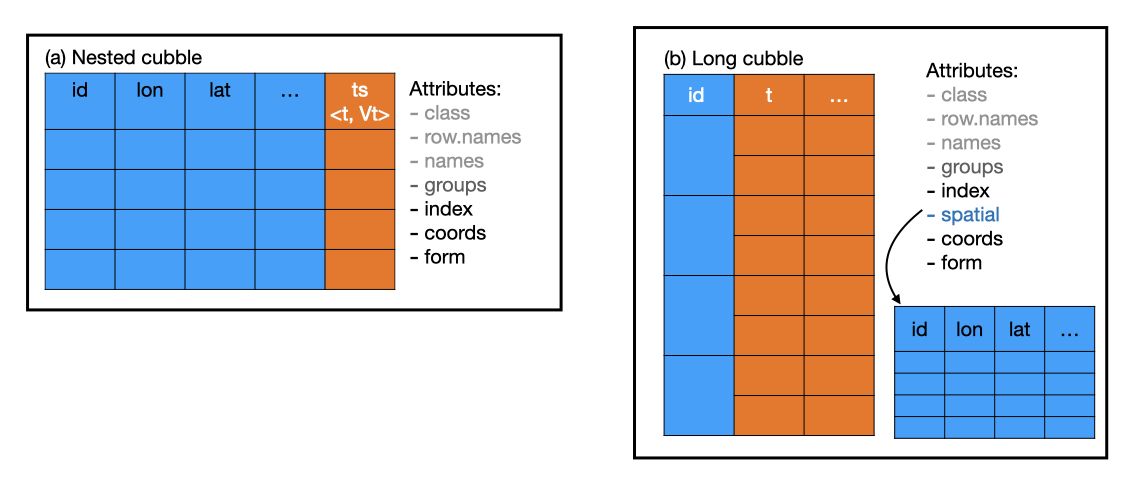
\includegraphics[width=1\linewidth,height=0.3\textheight]{/Users/sherryzhang/Documents/research/paper-cubble/figures/def-cubble/def-cubble.001} 

}

\caption[Illustration of nested and long cubble]{Illustration of nested and long cubble.}\label{fig:def-cubble}
\end{figure}
\end{CodeChunk}

\newpage

\hypertarget{create-a-cubble-in-the-nested-form}{%
\subsection{Create a cubble in the nested
form}\label{create-a-cubble-in-the-nested-form}}

To use functionalities from cubble, data analysts first need to create a
cubble. \texttt{as\_cubble} create a \texttt{cubble} by supplying the
three key components: \texttt{key} as the spatial identifier;
\texttt{index} as the temporal identifier; and a vector of
\texttt{coords} in the order of longitude first and then latitude. The
use of \texttt{key} and \texttt{index} follows the naming convention in
\texttt{tsibble}. The cubble created by default is in the nested form.
Below is an example of creating a cubble: \newline

\begin{CodeChunk}
\begin{CodeInput}
R> (cubble_nested <- cubble::climate_flat %>%
+   as_cubble(key = id, index = date, coords = c("long", "lat")))
\end{CodeInput}
\begin{CodeOutput}
# cubble:   id [5]: nested form
# bbox:     [115.97, -32.94, 133.55, -12.42]- check gap on long and lat
# temporal: date [date], prcp [dbl], tmax [dbl], tmin [dbl]
  id            lat  long  elev name           wmo_id ts                
  <chr>       <dbl> <dbl> <dbl> <chr>           <dbl> <list>            
1 ASN00009021 -31.9  116.  15.4 perth airport   94610 <tibble [366 x 4]>
2 ASN00010311 -31.9  117. 179   york            94623 <tibble [366 x 4]>
3 ASN00010614 -32.9  117. 338   narrogin        94627 <tibble [366 x 4]>
4 ASN00014015 -12.4  131.  30.4 darwin airport  94120 <tibble [366 x 4]>
5 ASN00015131 -17.6  134. 220   elliott         94236 <tibble [366 x 4]>
\end{CodeOutput}
\end{CodeChunk}

In the \texttt{cubble} header, you can read the name of the \texttt{key}
variable, bbox, and also the name of variable nested in the \texttt{ts}
column. In this example, the spatial identifier is \texttt{id} and the
number in the bracket means there are 5 unique \texttt{id} in this
dataset. The bbox in the second row gives the range of the coordinates.
The temporal variables are all nested in the \texttt{ts} column, but it
could be useful to know the name these variables. The third row in the
cubble header shows these names and in this example this includes:
precipitation, \texttt{prcp}, maximum temporature, \texttt{tmax}, and
minimum temperature, \texttt{tmin}.

\hypertarget{stretch-a-nested-cubble-into-the-long-form}{%
\subsection{Stretch a nested cubble into the long
form}\label{stretch-a-nested-cubble-into-the-long-form}}

From a created cubble in the nested form, analysts may want to directly
manipulate the temporal variables. This would require switching to the
long form using \texttt{stretch()}. The verb \texttt{stretch()} switch
the cubble from the nested form into a long form. Under the hood, it
first extracts the spatial variables into a separate tibble to store in
the attribute \texttt{spatial} and then unnests the \texttt{ts} column
to show the temporal content:

\begin{CodeChunk}
\begin{CodeInput}
R> (cubble_long <- cubble_nested %>% stretch(ts))
\end{CodeInput}
\begin{CodeOutput}
# cubble:  date, id [5]: long form
# bbox:    [115.97, -32.94, 133.55, -12.42]- check gap on long and lat
# spatial: lat [dbl], long [dbl], elev [dbl], name [chr], wmo_id [dbl]
   id          date        prcp  tmax  tmin
   <chr>       <date>     <dbl> <dbl> <dbl>
 1 ASN00009021 2020-01-01     0  31.9  15.3
 2 ASN00009021 2020-01-02     0  24.9  16.4
 3 ASN00009021 2020-01-03     6  23.2  13  
 4 ASN00009021 2020-01-04     0  28.4  12.4
 5 ASN00009021 2020-01-05     0  35.3  11.6
 6 ASN00009021 2020-01-06     0  34.8  13.1
 7 ASN00009021 2020-01-07     0  32.8  15.1
 8 ASN00009021 2020-01-08     0  30.4  17.4
 9 ASN00009021 2020-01-09     0  28.7  17.3
10 ASN00009021 2020-01-10     0  32.6  15.8
# ... with 1,820 more rows
\end{CodeOutput}
\end{CodeChunk}

Notice here that the third line in the header is changed to reflect the
spatial variables stored. This is a format suitable for computing
time-wise variables.

\hypertarget{tamp-a-long-cubble-back-to-the-nested-form}{%
\subsection{Tamp a long cubble back to the nested
form}\label{tamp-a-long-cubble-back-to-the-nested-form}}

Manipulation on the spatial and temporal dimension can be an iterative
process. Many times, we may decide to go back to the nested form after
some temporal manipulation. The verb to switch a long cubble back to the
nested form is \texttt{tamp()}:

\begin{CodeChunk}
\begin{CodeInput}
R> (cubble_back <- cubble_long %>% tamp())
\end{CodeInput}
\begin{CodeOutput}
# cubble:   id [5]: nested form
# bbox:     [115.97, -32.94, 133.55, -12.42]- check gap on long and lat
# temporal: date [date], prcp [dbl], tmax [dbl], tmin [dbl]
  id            lat  long  elev name           wmo_id ts                
  <chr>       <dbl> <dbl> <dbl> <chr>           <dbl> <list>            
1 ASN00009021 -31.9  116.  15.4 perth airport   94610 <tibble [366 x 4]>
2 ASN00010311 -31.9  117. 179   york            94623 <tibble [366 x 4]>
3 ASN00010614 -32.9  117. 338   narrogin        94627 <tibble [366 x 4]>
4 ASN00014015 -12.4  131.  30.4 darwin airport  94120 <tibble [366 x 4]>
5 ASN00015131 -17.6  134. 220   elliott         94236 <tibble [366 x 4]>
\end{CodeOutput}
\end{CodeChunk}

\hypertarget{migrate-spatial-variables-to-a-long-cubble}{%
\subsection{Migrate spatial variables to a long
cubble}\label{migrate-spatial-variables-to-a-long-cubble}}

As an output to be supplied to further visualisation or modelling,
analysts would usually like the spatial and temporal variables to be in
the same table. \texttt{migrate()} moves the spatial variables in the
attribute \texttt{spatial} into the long form cubble.

\begin{CodeChunk}
\begin{CodeInput}
R> (cubble_long %>% migrate(long, lat))
\end{CodeInput}
\begin{CodeOutput}
# cubble:  date, id [5]: long form
# bbox:    [115.97, -32.94, 133.55, -12.42]- check gap on long and lat
# spatial: lat [dbl], long [dbl], elev [dbl], name [chr], wmo_id [dbl]
   id          date        prcp  tmax  tmin  long   lat
   <chr>       <date>     <dbl> <dbl> <dbl> <dbl> <dbl>
 1 ASN00009021 2020-01-01     0  31.9  15.3  116. -31.9
 2 ASN00009021 2020-01-02     0  24.9  16.4  116. -31.9
 3 ASN00009021 2020-01-03     6  23.2  13    116. -31.9
 4 ASN00009021 2020-01-04     0  28.4  12.4  116. -31.9
 5 ASN00009021 2020-01-05     0  35.3  11.6  116. -31.9
 6 ASN00009021 2020-01-06     0  34.8  13.1  116. -31.9
 7 ASN00009021 2020-01-07     0  32.8  15.1  116. -31.9
 8 ASN00009021 2020-01-08     0  30.4  17.4  116. -31.9
 9 ASN00009021 2020-01-09     0  28.7  17.3  116. -31.9
10 ASN00009021 2020-01-10     0  32.6  15.8  116. -31.9
# ... with 1,820 more rows
\end{CodeOutput}
\end{CodeChunk}

\hypertarget{support-on-hierarchical-structure}{%
\subsection{Support on hierarchical
structure}\label{support-on-hierarchical-structure}}

\texttt{switch\_key()}

\hypertarget{support-on-interactive-graphics}{%
\subsection{Support on interactive
graphics}\label{support-on-interactive-graphics}}

\hypertarget{integrating-into-a-tidy-workflow}{%
\subsection{Integrating into a tidy
workflow}\label{integrating-into-a-tidy-workflow}}

Building from an underlying \texttt{tbl\_df} structure, it is natural to
implement methods available in \texttt{dplyr} to \texttt{cubble}.
Supported methods in the \texttt{cubble} with \texttt{dplyr} generics
includes:

\begin{center}
\begin{tabular}{ | m{5em} | m{15cm}| } 
\textbf{mutate} \\
\textbf{filter}\\
\textbf{summarise} \\
\textbf{select} \\
\textbf{arrange} \\
\textbf{rename} \\
\textbf{left\_join} \\
\textbf{group\_by} \\
\textbf{ungroup}\\
slice family & \textbf{slice\_head}, \textbf{slice\_tail}, \textbf{slice\_sample}, \textbf{slice\_min} and \textbf{slice\_max} \\
\end{tabular}
\end{center}

\texttt{cubble} is also compatible with \texttt{tsibble} in the sense
that the original list-column can be a \texttt{tbl\_ts} object.
Duplicates and gaps shoudl be first checked before structuring the data
into a cubble. If the input data is a \texttt{tsibble} object, the long
form cubble is also a \texttt{tsibble} where users can directly apply
time series operations.

\newpage

\hypertarget{examples}{%
\section{Examples}\label{examples}}

\hypertarget{australia-precipitation-pattern-in-2020}{%
\subsection{Australia precipitation pattern in
2020}\label{australia-precipitation-pattern-in-2020}}

Forming a cubble + basic tidyverse verbs - Vig 2 Aggregation - Vig 4

This vignette introduces how to perform spatial and temporal manipulate
in a cubble with dplyr verbs. We will illustrate with
\texttt{weatherdata::historical\_tmax} data, which have the historical
maximum temperature recorded for Australian stations with the earliest
dating back to 1859.

\hypertarget{spatial-manipulation}{%
\subsubsection{Spatial manipulation}\label{spatial-manipulation}}

\texttt{historical\_tmax} is already in a nested cubble format, which is
suitable for station-wise manipulation. \texttt{rnoaa} construct the
station id by prefix \texttt{ASN00} to the Bureau of Meteorology (BOM)
station number. In
\href{http://www.bom.gov.au/climate/cdo/about/site-num.shtml}{BOM's
numbering system}, the 2nd and 3rd digit denotes the state a station is
located in and this is equivalent to the 7th to 8th digit in our string.
We can mutate/ filter station in a particular state based on this
information and here we add a column called \texttt{state\_id} and
filter out the ones in New South Wales and Victoria (ranging from 46 to
90).

\begin{CodeChunk}
\begin{CodeInput}
R> tmax_nested <- weatherdata::historical_tmax %>%
+   mutate(state_id = stringr::str_sub(id, 7, 8)) %>%
+   filter(between(state_id, 46, 90))
\end{CodeInput}
\end{CodeChunk}

\hypertarget{temporal-manipulation}{%
\subsubsection{Temporal manipulation}\label{temporal-manipulation}}

There are some operations in the time dimension we would like to make:

\begin{itemize}
\tightlist
\item
  Extract observations in a particular period, say, those in 1971 to
  1975 and 2016 to 2020. This can be used to compare the historical and
  recent climate.
\item
  Summarise daily records into monthly to remove sparsity
\end{itemize}

These time dimension operations can be computed in the long form and
\texttt{stretch()} converts a nested cubble to a long cubble. From a
long cubble, we can write the exact same dplyr codes to complete the two
tasks:

\begin{CodeChunk}
\begin{CodeInput}
R> tmax_long <- tmax_nested %>%
+   stretch() %>%
+   filter(lubridate::year(date) %in% c(1971:1975, 2016:2020)) %>%
+   mutate(
+     month = lubridate::month(date),
+     group = as.factor(ifelse(
+       lubridate::year(date) > 2015,
+       "2016 ~ 2020",
+       "1971 ~ 1975"
+     ))
+   ) %>%
+   group_by(month, group) %>%
+   summarise(tmax = mean(tmax, na.rm = TRUE))
\end{CodeInput}
\end{CodeChunk}

\hypertarget{back-to-spatial}{%
\subsubsection{Back to spatial}\label{back-to-spatial}}

A data quality issue with the \texttt{rnoaa} data is that while it
records the first and last year recorded of each series, it doesn't
report the period of missingness. For example, station
\texttt{ASN00047048} starts it first record in 1957, pauses for a period
from 1963 to 1990, and then resumes it recording till today. Out of the
77 stations in New South Wales and Victoria, 7 stations have this issue
and we would like to remove those stations from the comparison.

Again, this is a station-wise operation and to convert back from the
long cubble to a nested one, use \texttt{tamp()}. Here we keep the
stations with 24 observations (12 months for both periods) after the
monthly aggregation.

\begin{CodeChunk}
\begin{CodeInput}
R> tmax_nested2 <- tmax_long %>%
+   tamp() %>%
+   filter(nrow(ts) == 24)
\end{CodeInput}
\end{CodeChunk}

In some visualisation, we may need information from both spatial and
temporal dimension. One example of this is a glyph map, where spatial
variables, i.e.~\texttt{longitude} and \texttt{latitude}, are used to
construct the major axes and temporal variables, i.e.~\texttt{month} and
\texttt{tmax}, are used to construct the minor axes. This requires these
variables to be in the same table, rather than in different forms. In
cubble, you can append spatial variables that are invariant to the
\texttt{key} withe \texttt{migrate()}

\begin{CodeChunk}
\begin{CodeInput}
R> tmax_long2 <- tmax_nested2 %>%
+   stretch() %>%
+   migrate(latitude, longitude)
\end{CodeInput}
\end{CodeChunk}

\hypertarget{glyph-map}{%
\subsubsection{Glyph map}\label{glyph-map}}

Now its time for the glyph map!

\begin{CodeChunk}
\begin{CodeInput}
R> gly <- glyphs(
+   tmax_long2,
+   x_major = "longitude",
+   y_major = "latitude",
+   x_minor = "month",
+   y_minor = "tmax",
+   height = 0.6,
+   width = 1
+ )
R> 
R> nsw_vic <- ozmaps::abs_ste %>%
+   filter(NAME %in% c("Victoria", "New South Wales"))
R> 
R> plot_map(nsw_vic, fill = "transparent") +
+   geom_path(data = gly, aes(gx, gy,
+     group = interaction(id, group),
+     color = group
+   )) +
+   scale_color_brewer(palette = "Dark2") + 
+   theme_bw() + 
+   coord_sf(xlim = c(140, 155)) + 
+   theme(legend.position = "bottom")
\end{CodeInput}


\begin{center}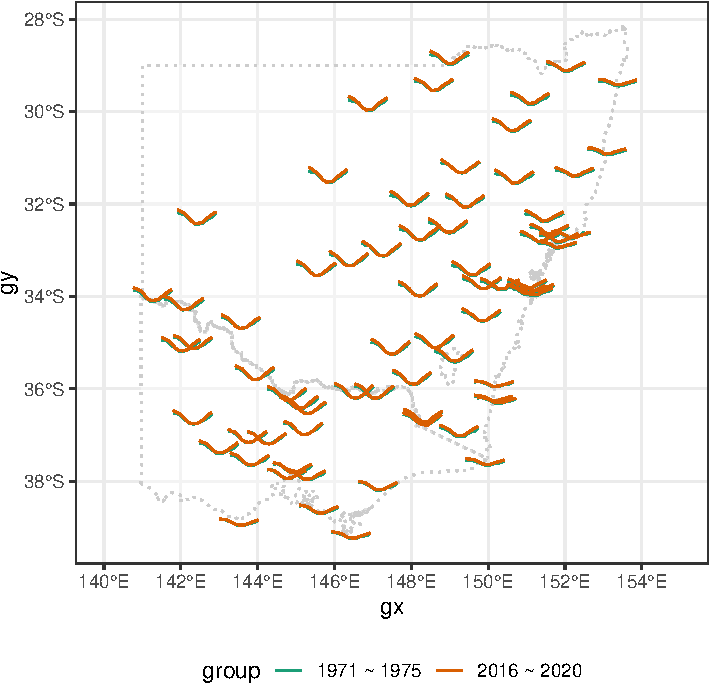
\includegraphics{figures/unnamed-chunk-10-1} \end{center}

\end{CodeChunk}

\hypertarget{spatial-and-temporal-aggregation}{%
\subsection{Spatial and temporal
aggregation}\label{spatial-and-temporal-aggregation}}

On top of \texttt{aus\_climate} data in this package,
\texttt{climate\_full} from package
\href{https://github.com/huizezhang-sherry/weatherdata}{\texttt{weatherdata}}
has daily climate data of 639 Australia stations from 2016 to 2020. This
is where these stations locate in an Australia map:

This is a lot of stations to look at for one climate variable and they
can't all fit into a glyph map. What we can do is to group stations into
clusters and look at the aggregated series in the glyph map. In this
vignette, I will introduce how to perform spatial (and temporal)
aggregation using hierarchical data structure in cubble.

First let's add a new column \texttt{ll} for calculating distance matrix
in the next section and aggregate the daily precipitation into weekly
measure. These steps should be familiar from the vignette \emph{Data
manipulation with cubble}.

\begin{CodeChunk}
\begin{CodeInput}
R> station_nested <- weatherdata::climate_full %>%
+   mutate(ll = s2::s2_lnglat(long, lat)) %>%
+   stretch() %>%
+   mutate(wk = lubridate::week(date)) %>%
+   group_by(wk) %>%
+   summarise(prcp = sum(prcp, na.rm = TRUE)) %>%
+   tamp()
\end{CodeInput}
\end{CodeChunk}

\hypertarget{hierarchical-data-structure}{%
\subsubsection{Hierarchical data
structure}\label{hierarchical-data-structure}}

Imposing a clustering structure can be thought of as building a
hierarchical structure where stations are nested within clusters. As an
example to illustrate here, we use a kmean clustering algorithm based on
the distance matrix and specify the number of centers to be 20. More
complex algorithms can also be used for more complex problem, as long as
a mapping from each station id to the cluster id can be constructed. We
then join this data to our station data:

\begin{CodeChunk}
\begin{CodeInput}
R> dist_raw <- scale(s2::s2_distance_matrix(station_nested$ll, station_nested$ll))
R> 
R> cluster_res <- tibble(
+   id = station_nested$id,
+   cluster = kmeans(dist_raw, centers = 20, nstart = 50)$cluster
+ )
R> 
R> station_nested <- station_nested %>%
+   left_join(cluster_res)
\end{CodeInput}
\end{CodeChunk}

One thing we hope to do with the cluster is to find the coordinates of
the centroid. These are variables variant to the station but invariant
to the cluster and it would be nice to have a function that structure
each cluster as a row. \texttt{switch\_key()} is the function that does
this: it lets you to specify a new key, say \texttt{cluster} and nests
all spatial variables variant to \texttt{cluster} into a column.
Temporal observations from different stations while within the same
cluster are bound in the nested column \texttt{ts}.

\begin{CodeChunk}
\begin{CodeInput}
R> cluster_nested <- station_nested %>%
+   switch_key(cluster)
\end{CodeInput}
\end{CodeChunk}

This structure makes it easy to compute cluster level variable, although
there are a few steps to calculate the centroid coordinates: we need to
find the convex hull that wraps around the cluster, make it a polygon,
find the centroid of the polygon and finally, extract the x and y
coordinate of each centroid:

\begin{CodeChunk}
\begin{CodeInput}
R> cluster_nested <- cluster_nested %>%
+   mutate(
+     chull = list(chull(.val$long, .val$lat)),
+     ll_cluster = sf::st_as_sfc(
+       s2::s2_make_polygon(c(.val$long[chull]),
+         c(.val$lat[chull]),
+         oriented = FALSE
+       )
+     ),
+     centroid = s2::s2_centroid(ll_cluster),
+     cent_long = s2::s2_x(centroid),
+     cent_lat = s2::s2_y(centroid)
+   )
\end{CodeInput}
\end{CodeChunk}

After we have got \texttt{cluster\_nested}, spatial and temporal data at
both levels can be easily obtained. If we use \texttt{station} and
\texttt{cluster} prefix to denote the two levels and \texttt{nested} and
\texttt{long} for whether the data shows the spatial or temporal
dimension, the relationship among the four datasets can be illustrated
in the following workflow:

Start with the original \texttt{station\_nested}, \texttt{stretch()}
expands the \texttt{ts} column with each station (\texttt{id}) forming a
group and attach variables invariant to \texttt{id} as an attribute.
\texttt{switch\_key()} changes the \texttt{key} from \texttt{id} to
\texttt{cluster} and nests all the spatial variables that variant to
\texttt{cluster}. \texttt{stretch()} \texttt{cluster\_nested} will store
variables that are invariant to \texttt{cluster} as a tibble in the
attribute.

Now we can obtain the aggregated series as described in the workflow
diagram above and construct the glyph map with
\texttt{GGally::glyphs()}:

\begin{CodeChunk}
\begin{CodeInput}
R> cluster_long <- cluster_nested %>%
+   stretch(ts) %>%
+   group_by(wk) %>%
+   summarise(prcp = sum(prcp, na.rm = TRUE)) %>%
+   migrate(cent_long, cent_lat)
R> 
R> gly <- GGally::glyphs(cluster_long,
+   x_major = "cent_long", x_minor = "wk",
+   y_major = "cent_lat", y_minor = "prcp",
+   height = 2, width = 4
+ )
R> 
R> state_map <- rmapshaper::ms_simplify(ozmaps::abs_ste, keep = 2e-3)
R> plot_map(state_map) +
+   geom_text(
+     data = cluster_nested,
+     aes(x = cent_long, y = cent_lat, label = cluster)
+   ) +
+   geom_path(
+     data = gly,
+     aes(x = gx, y = gy, group = gid)
+   )
\end{CodeInput}


\begin{center}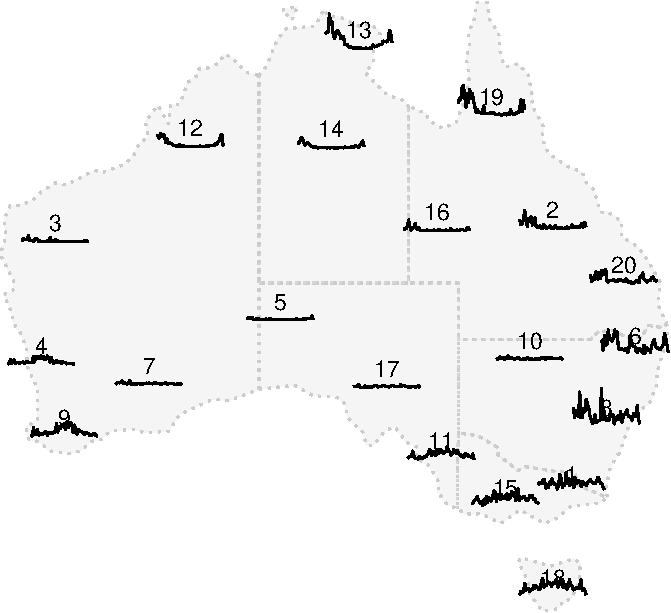
\includegraphics{figures/unnamed-chunk-15-1} \end{center}

\end{CodeChunk}

We can also look at the precipitation of each individual station within
the same cluster:

\begin{CodeChunk}
\begin{CodeInput}
R> station_long <- station_nested %>%
+   stretch(ts) %>%
+   migrate(cluster)
R> station_long %>%
+   ggplot(aes(x = wk, y = prcp, group = id)) +
+   geom_line(alpha = .3) +
+   facet_wrap(vars(cluster), scales = "free_y", ncol = 4) +
+   theme_bw()
\end{CodeInput}
\begin{figure}

{\centering 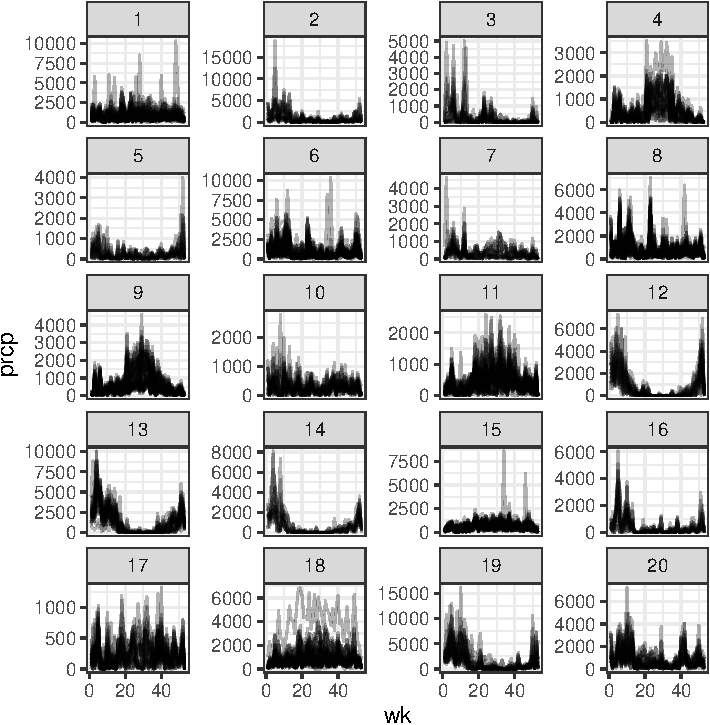
\includegraphics{figures/unnamed-chunk-16-1} 

}

\caption[shtishisa]{shtishisa}\label{fig:unnamed-chunk-16}
\end{figure}
\end{CodeChunk}

Lastly, there is one series on Tasmania island standing out from others,
lets look at where it is:

\begin{CodeChunk}
\begin{CodeInput}
R> # this part still needs some fixing
R> tas_latlong <- station_nested %>%
+   filter(lat < -40) %>%
+   mutate(p = max(ts$prcp)) %>%
+   strip_rowwise() %>%
+   filter(p == max(p))
R> 
R> state_map <- rmapshaper::ms_simplify(ozmaps::abs_ste, keep = 2e-3)
R> plot_map(state_map) +
+   geom_point(data = station_nested, aes(x = long, y = lat), size = 0.5) +
+   geom_sf(data = cluster_nested, aes(geometry = ll_cluster), fill = "transparent") +
+   geom_point(data = tas_latlong, aes(x = long, y = lat), col = "red")
\end{CodeInput}


\begin{center}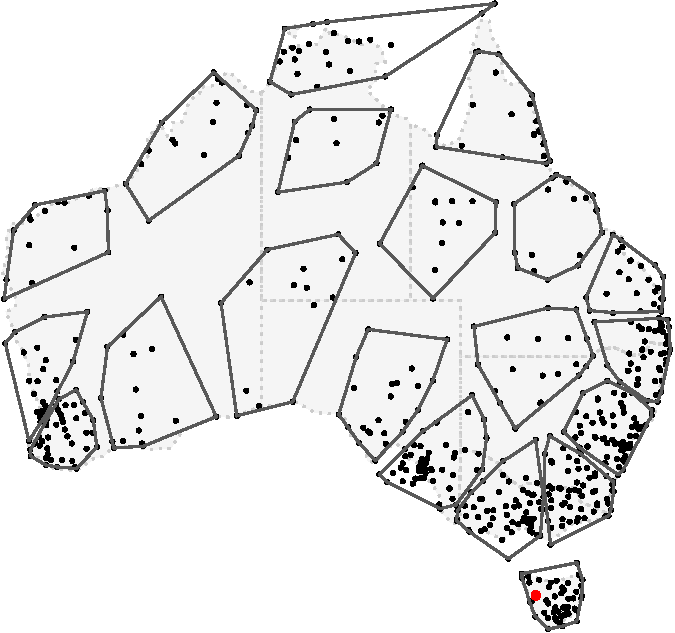
\includegraphics{figures/unnamed-chunk-17-1} \end{center}

\end{CodeChunk}

\hypertarget{matching-precipitation-and-river-level-in-victria-water-gauges}{%
\subsection{Matching precipitation and river level in Victria water
gauges}\label{matching-precipitation-and-river-level-in-victria-water-gauges}}

The water level data comes from
\href{http://www.bom.gov.au/metadata/catalogue/19115/ANZCW0503900528?template=full}{Bureau
of Meteorology} and has a copy in \texttt{weatherdata}. Here we extract
the water course level and add a column annotate this data of type
\texttt{river}. For the rainfall data, we will still use the
\texttt{weatherdata::climate\_full}, filtering for Victorian stations in
2020 should be pretty familiar by now. Again, we first look at where
these stations are on the map first:

\begin{CodeChunk}
\begin{CodeInput}
R> river <- weatherdata::water %>%
+   stretch() %>%
+   select(date, Water_course_level) %>%
+   tamp() %>%
+   mutate(type = "river")
R> 
R> climate <- weatherdata::climate_full %>%
+   filter(between(stringr::str_sub(id, 7, 8), 76, 90)) %>%
+   stretch() %>%
+   filter(lubridate::year(date) == 2020) %>%
+   tamp() %>%
+   mutate(type = "climate")
R> 
R> vic_map <- rmapshaper::ms_simplify(ozmaps::abs_ste %>% filter(NAME == "Victoria"))
R> plot_map(vic_map) +
+   geom_point(
+     data = dplyr::bind_rows(river, climate),
+     aes(x = long, y = lat, color = type)
+   ) +
+   scale_color_brewer(palette = "Dark2") +
+   theme_bw()
\end{CodeInput}


\begin{center}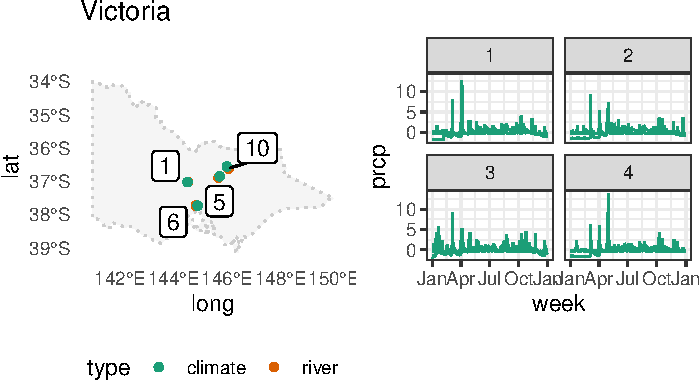
\includegraphics{figures/unnamed-chunk-18-1} \end{center}

\end{CodeChunk}

\hypertarget{theory}{%
\subsubsection{Theory}\label{theory}}

Temporal matching checks how spatially matched pairs align temporally.
We use the following chart to illustrate how the temporal matching
works:

\begin{CodeChunk}
\begin{figure}

{\centering 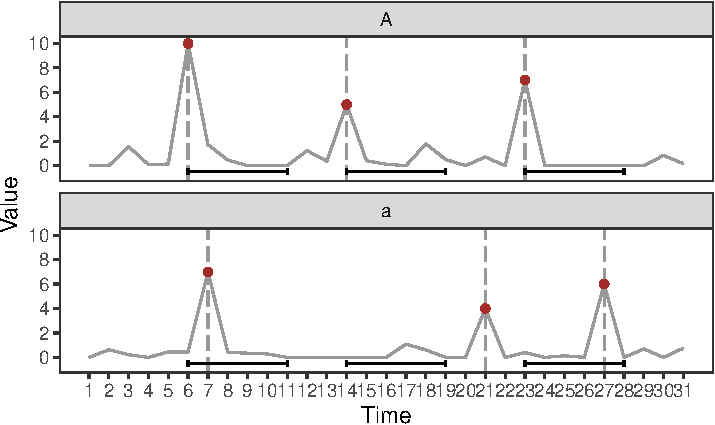
\includegraphics{figures/unnamed-chunk-19-1} 

}

\caption[shtishisaasdf]{shtishisaasdf}\label{fig:unnamed-chunk-19}
\end{figure}
\end{CodeChunk}

For each spatially matched pair, say \texttt{A} and \texttt{a}, we first
find the largest \texttt{n} points in each series, colored in brown
points here. Here we use the largest three but you can tune this number
by \texttt{temporal\_n\_highest}. Then we construct the interval of the
largest points from one series and see how many points, from the other
series, fall into the intervals. The series used to construct the
interval is controlled by \texttt{temporal\_independent} and the window
size by \texttt{temporal\_window} with a default of 5.

In this illustration, we construct the interval based on series
\texttt{A} and two of the three peaks from \texttt{a} falls into this
interval at Time 7 and 27.

\hypertarget{rainfall-translates-into-river-level}{%
\subsubsection{Rainfall translates into river
level}\label{rainfall-translates-into-river-level}}

There's another mandatory argument that hasn't been introduced above:
\texttt{temporal\_var\_to\_match}. This argument controls the variable
to match and it needs to appear in both the \texttt{major} and
\texttt{minor} set. In the water level matching example, we match the
variable \texttt{Water\_course\_level} from \texttt{river} to
\texttt{prcp} from \texttt{climate}, hence need to manually rename one
of them to match the other, here we rename \texttt{Water\_course\_level}
to \texttt{prcp} in \texttt{river}:

\begin{CodeChunk}
\begin{CodeInput}
R> river <- river %>%
+   stretch() %>%
+   rename(prcp = Water_course_level) %>%
+   tamp()
\end{CodeInput}
\end{CodeChunk}

Now we use \texttt{match\_sites()} to first pair the weather stations
with the river gauges spatially and then apply the temporal matching on
\texttt{prcp}. We will construct the interval based on peaks in
\texttt{climate} since we would expect a lag effect for precipitation to
flow into the river and cause a raise in river level, hence
\texttt{temporal\_independent\ =\ climate}. We select the 30 highest
peak from the series to construct the match by setting
\texttt{temporal\_n\_highest\ =\ 30}. This is a tuning parameter and you
can start with 10\% of the points of one series (here we have daily data
for a year, 10\% is roughly 30 points). \texttt{temporal\_min\_match}
filters out pairs don't have enough match and to return all the pairs,
set \texttt{temporal\_min\_match} to \texttt{0}.

\begin{CodeChunk}
\begin{CodeInput}
R> res <- match_sites(river, climate,
+   temporal_var_to_match = prcp,
+   temporal_independent = climate,  
+   temporal_n_highest = 30,
+   temporal_min_match = 15
+ )
R> 
R> res
\end{CodeInput}
\begin{CodeOutput}
# cubble:   id [8]: nested form
# bbox:     [144.52, -37.73, 146.06, -36.55]
# temporal: date [date], prcp [dbl]
  id          name                lat  long type  ts        .dist .group n_match
  <chr>       <chr>             <dbl> <dbl> <chr> <list>    <dbl>  <int>   <int>
1 405234      SEVEN CREEKS @ D~ -36.9  146. river <tibble ~  6.15      5      21
2 ASN00082042 strathbogie       -36.8  146. clim~ <tibble ~  6.15      5      21
3 404207      HOLLAND CREEK @ ~ -36.6  146. river <tibble ~  8.54     10      21
4 ASN00082170 benalla airport   -36.6  146. clim~ <tibble ~  8.54     10      21
5 230200      MARIBYRNONG RIVE~ -37.7  145. river <tibble ~  6.17      6      19
6 ASN00086038 essendon airport  -37.7  145. clim~ <tibble ~  6.17      6      19
7 406213      CAMPASPE RIVER @~ -37.0  145. river <tibble ~  1.84      1      18
8 ASN00088051 redesdale         -37.0  145. clim~ <tibble ~  1.84      1      18
\end{CodeOutput}
\end{CodeChunk}

The output from temporal matching is also a cubble, with additional
column \texttt{.dist} and \texttt{.group} inherent from spatial matching
and \texttt{n\_match} for the number of matched temporal peaks. Then you
can use this output to plot the location of match or to look at the
series:

\begin{CodeChunk}
\begin{CodeInput}
R> p1 <- plot_map(vic_map) +
+   geom_point(
+     data = res,
+     aes(x = long, y = lat, color = type)
+   ) +
+   ggrepel::geom_label_repel(
+     data = res %>% filter(type == "river"),
+     aes(x = long, y = lat, label = .group)
+   ) +
+   scale_color_brewer(palette = "Dark2") +
+   ggtitle("Victoria") +
+   theme_minimal() +
+   theme(
+     panel.grid.major = element_blank(),
+     panel.grid.minor = element_blank(),
+     legend.position = "bottom"
+   )
R> 
R> res_long <- res %>%
+   stretch(ts) %>%
+   migrate(.group, type) %>%
+   mutate(prcp = scale(prcp)[, 1]) %>%
+   switch_key(.group) %>%
+   migrate(type)
R> 
R> p2 <- res_long %>%
+   ggplot(aes(
+     x = date, y = prcp,
+     group = id, color = type
+   )) +
+   geom_line() +
+   facet_wrap(vars(.group)) +
+   scale_color_brewer(palette = "Dark2", guide = "none") +
+   theme_bw() +
+   labs(x = "week") +
+   scale_x_date(date_labels = "%b")
R> 
R> p1 | p2
\end{CodeInput}
\begin{figure}

{\centering 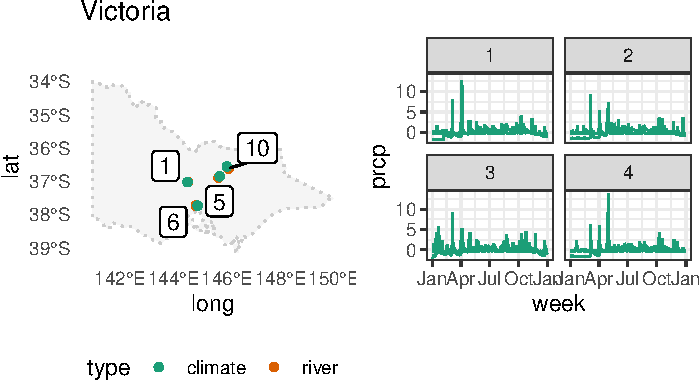
\includegraphics[width=1\linewidth]{figures/unnamed-chunk-22-1} 

}

\caption[..]{...}\label{fig:unnamed-chunk-22}
\end{figure}
\end{CodeChunk}

\hypertarget{interative-graphic-with-cubble}{%
\subsection{Interative graphic with
cubble}\label{interative-graphic-with-cubble}}

\begin{CodeChunk}
\begin{CodeInput}
R> set.seed(123)
R> tmax_data <- weatherdata::climate_full %>%
+   slice_sample(n = 50) %>%
+   stretch() %>%
+   mutate(ym = tsibble::yearmonth(date)) %>%
+   group_by(ym) %>%
+   summarise(
+     tmax = mean(tmax, na.rm = TRUE),
+     tmin = mean(tmin, na.rm = TRUE),
+     prcp = sum(prcp, na.rm = TRUE)
+   ) %>%
+   ungroup(ym) %>%
+   mutate(
+     year = as.factor(year(ym)),
+     month = as.factor(month(ym)),
+     prcp = sqrt(prcp + 0.001)
+   ) %>%
+   tamp() %>%
+   mutate(median_tmax = median(ts$tmax, na.rm = TRUE)) %>%
+   stretch() %>%
+   migrate(median_tmax, long, lat, name) %>%
+   highlight_key(~id)
R> 
R> p1 <- tmax_data %>%
+   ggplot(aes(
+     x = month, y = tmax, group = interaction(year, id),
+     color = median_tmax, label = name
+   )) +
+   geom_line() +
+   facet_wrap(vars(fct_reorder(name, -median_tmax))) +
+   theme(legend.position = "none")
R> 
R> state_map <- rmapshaper::ms_simplify(ozmaps::abs_ste, keep = 2e-3)
R> p2 <- tmax_data %>%
+   ggplot() +
+   geom_sf(data = state_map, aes(geometry = geometry)) +
+   geom_point(aes(x = long, y = lat, color = median_tmax, label = name)) +
+   theme_void()
R> 
R> bscols(
+   ggplotly(p1, width = 800, height = 800, tooltip = "label") %>%
+     highlight(on = "plotly_selected", off = "plotly_deselect", color = "red"),
+   ggplotly(p2, width = 800, height = 800, tooltip = "label") %>%
+     highlight(on = "plotly_selected", off = "plotly_deselect", color = "red")
+ )
\end{CodeInput}
\end{CodeChunk}

\hypertarget{conclusion}{%
\section{Conclusion}\label{conclusion}}

\newpage

\hypertarget{old-stuff}{%
\section{Old stuff}\label{old-stuff}}

Many spatial and spatio-temporal data structures have been developed by
the R-spatial team for both raster and vector spatial data. For vector
spatial data, which is the focus of this paper, \texttt{sf}
\citep{pebesma2018simple} represents spatial vector information with
simple features: points, lines, polygons and their multiples. Various
\texttt{st\_} function are designed to manipulate these features based
on their geometric relationships. For spatio-temporal data,
\texttt{stars} \citep{stars} can represent both raster and vector data
using multi-dimensional array. However, the underlying array structure
can be difficult to operate for data analysts who are more familiar with
a flat 2D data frame structure used by the tidyverse ecosystem.

In the temporal aspect, the \texttt{tsibble} \citep{tsibbles} structure
and its tidyverts ecosystem have provided a {[}\ldots{} {]} workflow to
work with temporal data. In a tsibble structure, temporal data is
characterised by \texttt{index} and \texttt{key} where \texttt{index} is
the temporal identifier and \texttt{key} is the identifier for multiple
series, which could be used as a spatio identifier. However, a tsibble
object, by construction, always requires the \texttt{index} in its
structure. This makes it less appealing for spatio-temporal data since
the output of calculated spatio-specific variables (i.e.~features of
each series) don't have the time dimension. Analysts will either need to
have an additional step to join this output to the original tsibble or
operate with variables stored in two separate objects. In addition, the
long form structure of a tsibble object means spatio variables
(i.e.~longitude, latitude, and features of each series if joined back to
the tsibble) of each spatio identifier will be repetitively recorded at
each timestamp. This repetition is unnecessary and would inflate the
object size for long series.

\hypertarget{a-new-data-structure-for-spatio-temporal-data}{%
\section{A new data structure for spatio-temporal
data}\label{a-new-data-structure-for-spatio-temporal-data}}

\textbf{The main difficulty and challenge}\\
The main difficulty in visualising this type of data is to show
information in both space and time dimension with the proper level of
details without information overflow. This would sometimes require
aggregating the time dimension into the proper level or slicing the data
into a reasonable number of subset for display. In this sense, a data
structure that regulates the manipulation spatio-temporal data will
benefit the analysis workflow. While many implementations focus on
manipulating and visualising pure spatial or temporal data, there are
not sufficient tools to deal with spatio-temporal data. The purpose of
this paper is to introduce a spatio-temporal vector data structure for
data analysis in R.

To work with spatio-temporal data, analysts can choose to either work
separately on each dimension or join the two sets together, however,
each approach has its own problem: While is is natural to work
separately on each sheet (since spatial and temporal operations usually
don't overlap), analysts will need to manually keep the other data frame
up to date. For example, the following pseudo code illustrates the
scenario where once the spatial dataset is filtered for those within
Victoria, the temporal dataset needs to be manually updated to reflect
this spatial filter.

\begin{CodeChunk}
\begin{CodeInput}
R> spatial_new <- spatial %>% filter(SITES_IN_VICTORIA)
R> temporal_new <- temporal %>% filter(id %in% spatial_new$id)
\end{CodeInput}
\end{CodeChunk}

If analysts choose to join the spatial and temporal data together, the
joined dataset could be too large since each spatial variable will be
repeated at each time stamp for each site. Also, recordings of the site
ID from different data sources can be slightly different from each
other, causing a painful checking and cleaning of site IDs before the
join.

\newpage

\hypertarget{create-a-cubble}{%
\section{Create a cubble}\label{create-a-cubble}}

The creation of a cubble requires the site identifier (\texttt{key}), as
well as the spatial (\texttt{coords}) and temporal (\texttt{index})
identifier. \texttt{climate\_flat} is already a tibble and it uses
\texttt{id} to identify each station, \texttt{date} as the time
identifier, and \texttt{c(long,\ lat)} as the spatial identifier. To
create a cubble for this data, use:

\begin{CodeChunk}
\begin{CodeInput}
R> climate_flat %>% as_cubble(key = id, index = date, coords = c(long, lat))
\end{CodeInput}
\begin{CodeOutput}
# cubble:   id [5]: nested form
# bbox:     [115.97, -32.94, 133.55, -12.42]- check gap on long and lat
# temporal: date [date], prcp [dbl], tmax [dbl], tmin [dbl]
  id            lat  long  elev name           wmo_id ts                
  <chr>       <dbl> <dbl> <dbl> <chr>           <dbl> <list>            
1 ASN00009021 -31.9  116.  15.4 perth airport   94610 <tibble [366 x 4]>
2 ASN00010311 -31.9  117. 179   york            94623 <tibble [366 x 4]>
3 ASN00010614 -32.9  117. 338   narrogin        94627 <tibble [366 x 4]>
4 ASN00014015 -12.4  131.  30.4 darwin airport  94120 <tibble [366 x 4]>
5 ASN00015131 -17.6  134. 220   elliott         94236 <tibble [366 x 4]>
\end{CodeOutput}
\end{CodeChunk}

Most of the time, spatio-temporal data doesn't come into this form and
analysts need to query the climate variables based on station metadata.
\textcolor{red}{This is also a problem illustrated in Section 3.5 in @tidydata. Here we provide a structured way to query this data based on the row-wise operator and nested list.}
For this type of task, one can structure a metadata into a tibble and
use row-wise operator to query the climate variables into a nested list.
As an example here we demonstrate the workflow to find the 5 closest
stations to Melbourne. We first create a station data frame with the 5
target stations.

\begin{CodeChunk}
\begin{CodeOutput}
# A tibble: 5 x 8
  id            lat  long  elev name                 wmo_id  dist city     
  <chr>       <dbl> <dbl> <dbl> <chr>                 <dbl> <dbl> <chr>    
1 ASN00086038 -37.7  145.  78.4 essendon airport      95866  10.8 melbourne
2 ASN00086282 -37.7  145. 113.  melbourne airport     94866  20.1 melbourne
3 ASN00086077 -38.0  145.  12.1 moorabbin airport     94870  21.9 melbourne
4 ASN00088162 -37.4  145. 528.  wallan (kilmore gap)  94860  48.1 melbourne
5 ASN00087113 -38.0  144.  10.6 avalon airport        94854  48.8 melbourne
\end{CodeOutput}
\end{CodeChunk}

We can query the climate information into a nested list named
\texttt{ts} for each station with the \texttt{rowwise()} operator. To
create a cubble, supply the same identifiers as with the first example.

\begin{CodeChunk}
\begin{CodeInput}
R> sydmel_climate <- stations %>%
+   rowwise() %>%
+   mutate(ts = list(meteo_pull_monitors(id,
+     date_min = "2020-01-01",
+     date_max = "2020-12-31",
+     var = c("PRCP", "TMAX", "TMIN")
+   ) %>%
+     select(-id))) %>%
+   as_cubble(key = id, index = date, coords = c(long, lat))
\end{CodeInput}
\end{CodeChunk}

\begin{CodeChunk}
\begin{CodeOutput}
# cubble:   id [5]: nested form
# bbox:     [144.47, -38.03, 145.1, -37.38]
# temporal: date [date], prcp [dbl], tmax [dbl], tmin [dbl]
  id            lat  long  elev name                 wmo_id  dist city   ts     
  <chr>       <dbl> <dbl> <dbl> <chr>                 <dbl> <dbl> <chr>  <list> 
1 ASN00086038 -37.7  145.  78.4 essendon airport      95866  10.8 melbo~ <tibbl~
2 ASN00086282 -37.7  145. 113.  melbourne airport     94866  20.1 melbo~ <tibbl~
3 ASN00086077 -38.0  145.  12.1 moorabbin airport     94870  21.9 melbo~ <tibbl~
4 ASN00088162 -37.4  145. 528.  wallan (kilmore gap)  94860  48.1 melbo~ <tibbl~
5 ASN00087113 -38.0  144.  10.6 avalon airport        94854  48.8 melbo~ <tibbl~
\end{CodeOutput}
\end{CodeChunk}

Below are the how the nested and long form look like for Australia
climate data, which records daily precipitation, maximum and minimum
temperature for 55 stations across Australia from 2015- 2020. Notice
that each station forms a group in both forms and specifically, the
nested and long form have a underlying \texttt{rowwise\_df} and
\texttt{grouped\_df} respectively.

With a cubic framework on mind, different types of manipulation with
cubble can be thought of as slicing the cube in various way. The table
below shows how some \texttt{dplyr} verbs are mapped into the operation
in a cubble. With the existing grouping on the station, additional
groupping can be added with \texttt{group\_by} and removed with
\texttt{ungrouped}. {[}talk about why it is useful{]}

\newpage

\hypertarget{cubble-operations}{%
\subsection{Cubble operations}\label{cubble-operations}}

\begin{CodeChunk}
\begin{figure}

{\centering 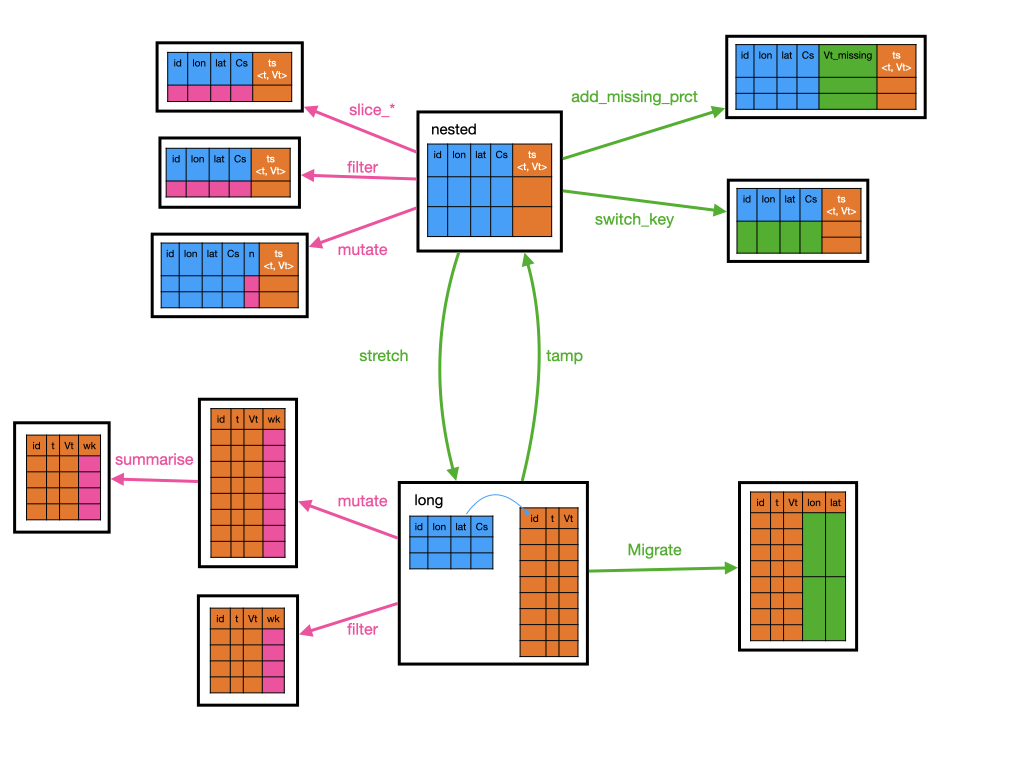
\includegraphics[width=0.9\linewidth,height=0.5\textheight]{/Users/sherryzhang/Documents/research/paper-cubble/figures/cubble-operations/cubble-operations.001} 

}

\caption[Cubble operations]{Cubble operations}\label{fig:cubble-operations}
\end{figure}
\end{CodeChunk}

\hypertarget{basics}{%
\subsubsection{Basics}\label{basics}}

\begin{itemize}
\tightlist
\item
  \texttt{stretch}: nest to long form
\item
  \texttt{tamp}: long to nest form
\item
  \texttt{migrate}: move selected spatial variables to the long form.
\item
  \texttt{add\_dscrb\_prct}: summary stats for missingness
\end{itemize}

dplyr compatibility:

\begin{itemize}
\tightlist
\item
  mutate, filter, summarise, select, arrange
\item
  group and ungroup: group\_by, ungroup
\item
  slice family
\end{itemize}

\hypertarget{combine-two-cubbles}{%
\subsubsection{Combine two cubbles}\label{combine-two-cubbles}}

\begin{itemize}
\tightlist
\item
  match river and weather gauges data
\item
  involve combining two cubbles
\item
  join operations combine the two together by appending more rows but
  what we really want is to bind rows.
\item
  bind rows also doesn't work since we want to bind only when there' s a
  matching????
\item
  introduce bind\_join
\end{itemize}

\hypertarget{hierarchical-structure-in-cubble}{%
\subsubsection{Hierarchical structure in
cubble}\label{hierarchical-structure-in-cubble}}

\begin{itemize}
\tightlist
\item
  hierarchical is common.
\item
  Given examples.
\item
  Essence: switch between different levels
\item
  introduce \texttt{switch\_key}
\end{itemize}

\hypertarget{examples-1}{%
\section{Examples}\label{examples-1}}

Daily climate data (prcp, tmax, and tmin) from RNOAA - lots of stations
across Australia

An exploratory data analysis questions: What's the climate profile look
like in Australia

\begin{itemize}
\tightlist
\item
  General features: Any general trend/ fluctuation in prcp, tmax, and
  tmin?
\item
  Local features: Any station stands out from the crowd?
\end{itemize}

\bibliography{references.bib}


\end{document}
